
\documentclass{abgabe}
\begin{document}

\begin{questions}
    \qformat{\thequestion. \textbf{\thequestiontitle} \hfill}
    \titledquestion{Lastenheft Fahrkartenautomat}
    In dieser Aufgabe soll eine erste Version des Lastenheftes für den Fahrkartenautomat entwickelt werden. Ein Fahrkartenautomat kann wie folgt benutzt werden:

    Kunden können mit dem Automaten Fahrkarten kaufen.
    Dabei kann der Kunde den Kaufvorgang jederzeit abbrechen (modellieren Sie diesen Fall als \gqq{Erweiterung} eines Anwendungsfalles).
    Der Automat schickt regelmäßig eine Anfrage an den Server der Verkehrsbetriebe, um die aktuellen Preisdaten abzufragen.
    Außerdem verschickt der Automat an den Server Warnungen und Fehlernachrichten.
    Alle bisher beschriebenen Aktivitäten soll der Automat protokollieren.

    Das Servicepersonal der Verkehrsbetriebe muss regelmäßig Papier und Farbbänder an dem Automat nachfüllen.
    Die Verkehrsbetriebe haben außerdem einen Administrator, der sich die Protokolle des Automaten über eine Internetverbindung anschauen kann.
    Zusätzlich kann er den Münzspeicher auslesen, die Software-Version auslesen, oder den ganzen Automaten deaktivieren.
    Für alle Tätigkeiten muss sich der Administrator erst am Automat anmelden.

    \href{https://www.ili.fh-aachen.de/goto_elearning_file_403173_download.html}{Hier} finden Sie ein Rahmengerüst für ein Lastenheft, das auch ein Glossar der wichtigsten Begriffe enthält.
    \emph{Dieses Glossar ist nur als Grundgerüst vorhanden, und soll während der Bearbeitung der folgenden Unterpunkte stetig aktualisiert werden.}
    Wenn also ein Begriff verwendet wird, der erklärt werden sollte, muss das Glossar entsprechend erweitert werden.

    Erstellen Sie das Lastenheft für den Fahrkartenautomat:
    \begin{enumerate}
        \item Bestimmen Sie mögliche \emph{Stakeholder} des Projekts und notieren Sie deren \emph{Ziele} als kurzen Text.
        \item Strukturieren Sie das System mit Hilfe eines \emph{Use-Case-Diagrammes}, das auf dem in der Einführung angegebenen Text basiert.
              Fügen Sie an der entsprechenden Stelle ihr Resultat als Abbildung ein.
        \item Dokumentieren Sie den Anwendungsfall „Fahrkarte kaufen“ im Detail, d.h. füllen Sie die entsprechende \emph{Schablone für Anwendungsfälle  (textuelle Beschreibungen der Use-Cases)} aus.
        \item Dokumentieren Sie 2-3 weitere Anwendungsfälle aus Unterpunkt 2. Eine grobe Beschreibung der typischen und alternativen Abläufe reicht hier.
        \item Überlegen Sie sich 2-3 realistische, \emph{nicht-funktionale Anforderungen}.
        \item Zur Klärung der Detailanforderungen mit den Verkehrsbetrieben soll ein \emph{UI-Prototyp} der \emph{Nutzeroberfläche} für den \emph{Administrator} entworfen werden.
              Gehen Sie davon aus, dass das \emph{Login bereits erfolgt} ist.
              Ein Mockup gehört zu den \emph{nicht-funktionalen} Anforderungen.
    \end{enumerate}

    Halten Sie diese Informationen im Lastenheft fest.

    Verwenden Sie für das Use-Case Diagramm und den UI-Mockup z.B. das Programm \href{https://www.ili.fh-aachen.de/ilias.php?baseClass=ilLinkResourceHandlerGUI&ref_id=341847&cmd=calldirectlink}{Visual Paradigm}. Für das UI Mockup können Sie in Visual Paradigm den Diagrammtypen "Wireframe" verwenden.
    Die Nutzeroberfläche soll ohne Flows auskommen und nur aus einer Seite bestehen, aber alle Funktionalitäten enthalten.

    \clearpage

    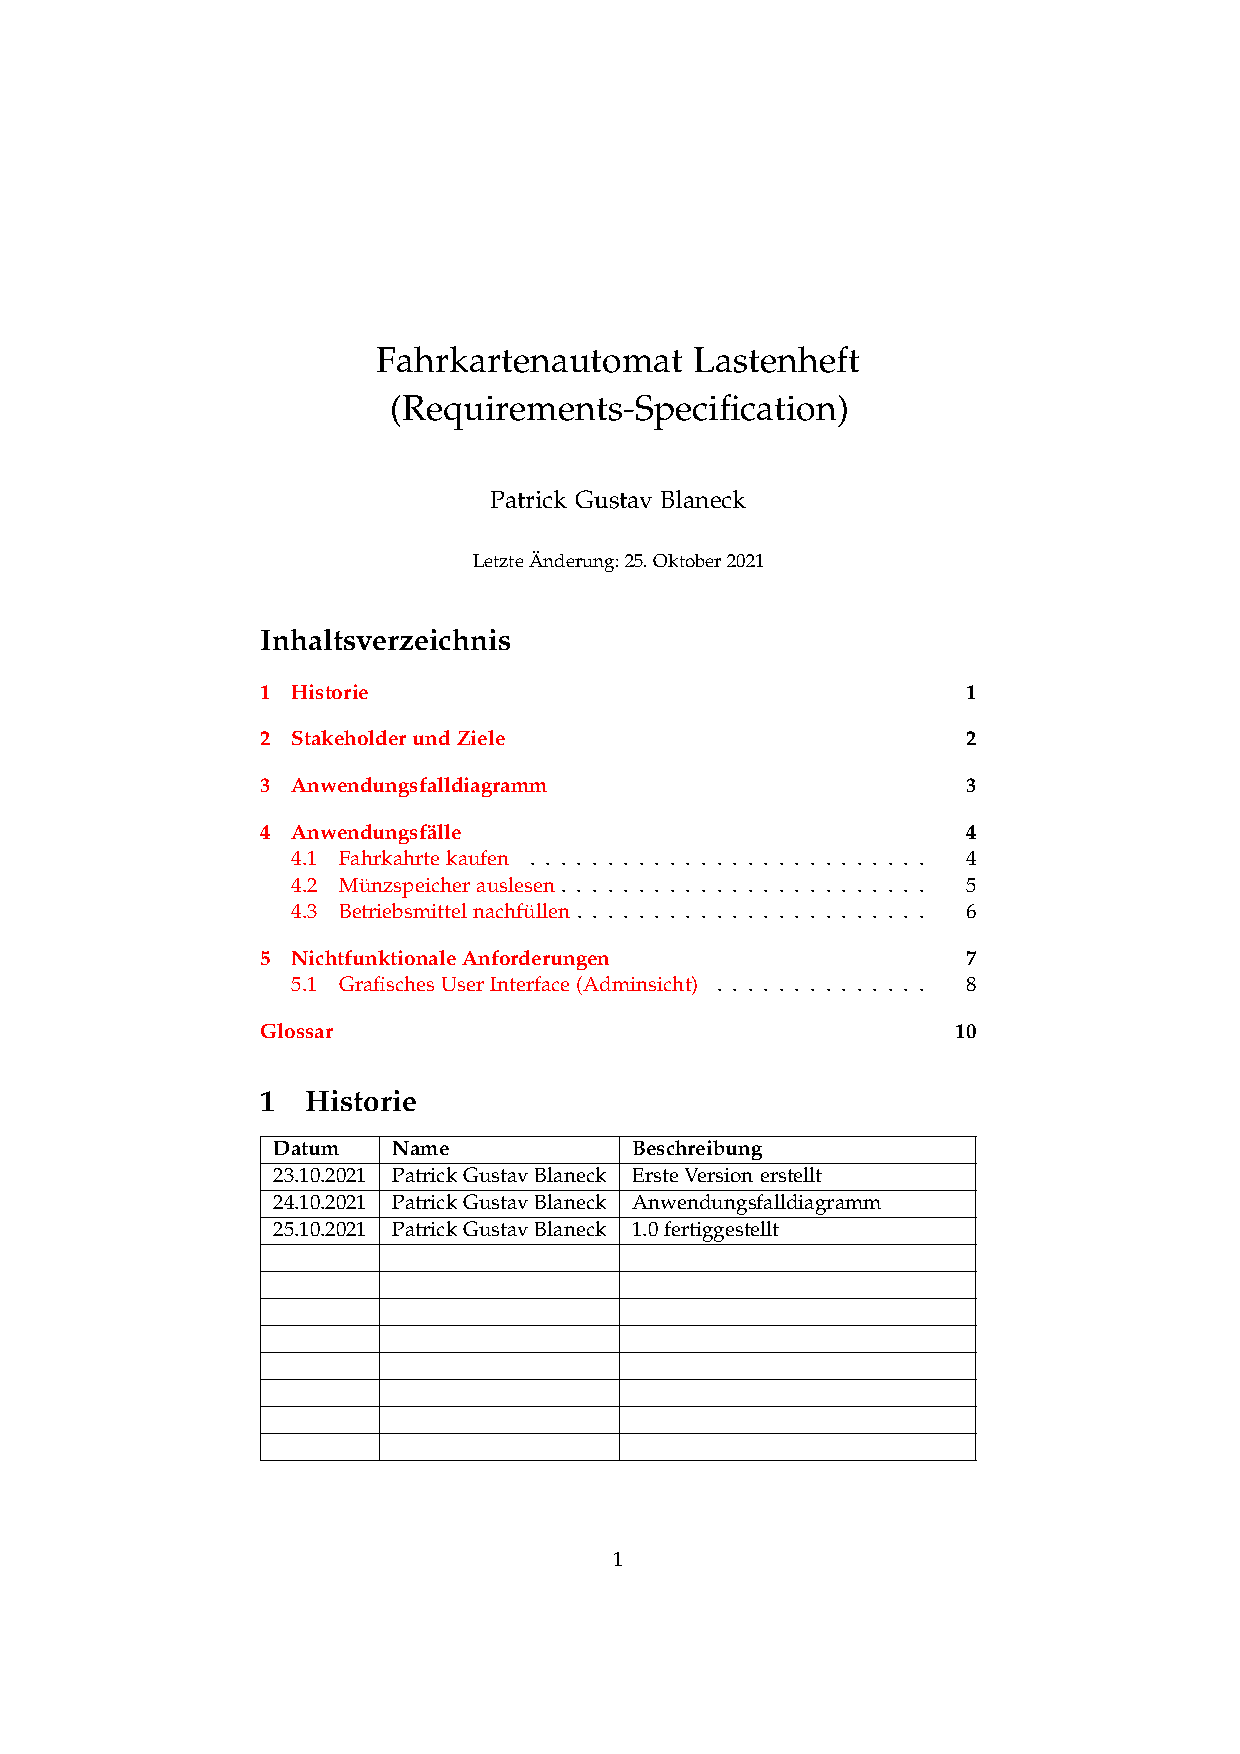
\includepdf[pages=-]{swt_blaneck_patrick_h03_lastenheft.pdf}
\end{questions}
\end{document}